%font size,paper size,   text_type=book, report, article, scrreprt
\documentclass[11pt,a4paper,oneside]{article}
%text encoding to output additional symbols (ö,ä,ü,ß,...)
\usepackage[T1]{fontenc}
%text encoding to input additional symbols (ö,ä,ü,ß,...)
\usepackage[utf8]{inputenc}
%language for captions,time format,...
\usepackage[english,main=ngerman]{babel}
%for xelatex & lualatex to import other fonts
\usepackage{fontspec}
%latin modern font (sharp letters)
\usepackage{lmodern}
%imidiate pagebreak
\raggedbottom
%include pdf
\usepackage{pdfpages}

%additional math enviroments (equation,align,multline,alignat), functions (\sin,\lim)
\usepackage{amsmath}
%additional math fonts (\mathbb{},\mathbf{},\mathcal{},...)
\usepackage{amsfonts}
%additional math symbols
\usepackage{amssymb}
%additional symbols (\de­gree,\cel­sius,\pert­hou­sand,\mi­cro,\ohm)
\usepackage{gensymb}
%different integral simbols: \iiint \oint
\usepackage{ulem}\usepackage[upint]{stix}
%good formated data with error in math enviroment
\usepackage[separate-uncertainty=true]{siunitx}
%nice looking fractions
\usepackage{xfrac}
%cirlces around text
\usepackage{tikz}
\newcommand\encircle[1]{%
  \tikz[baseline=(X.base)] 
    \node (X) [draw, shape=circle, inner sep=0] {\strut #1};}
%boxes for code
\usepackage{listings}

%include pictures
\usepackage{graphicx}
%image/table wrapper for floating images/tables between text
\usepackage{wrapfig}
%other figure wrapper
\usepackage{subfigure}
%better footnote enviroment
\usepackage{footnote}
%add links
%\usepackage{hyperref}
%multiline comments
\usepackage{comment}

%colors (base): black, cyan, green, orange, violet, blue, darkgray, lightgray, purple, white, brown, gray, magenta, red, yellow,
%colors (additional 68)  with [dvipsnames]: https://www.namsu.de/Extra/pakete/Xcolor.html
%\usepackage[dvipsnames]{xcolor}
\usepackage{xcolor}

%define document borders
\usepackage[left=2cm,right=2cm,top=2cm,bottom=2cm]{geometry}
%indent (einrücken)
\setlength{\parindent}{0pt}
%disable uppercase 
\newcommand{\RM}[1]{\MakeUppercase{\romannumeral #1{}}}
%define shortcuts for images & tables
\addto\captionsngerman{
\renewcommand{\figurename}{Abb.}
\renewcommand{\tablename}{Tab.}}

%disable numbering of equations:
%\makeatletter
%\renewcommand\tagform@[1]{}
%\makeatother

%select different font
%\usepackage{xfrac,fontspec,unicode-math}
%\newfontfamily{\headingsfont}{Segoe Print}
%\addtokomafont{disposition}{\headingsfont\color{blue}}
%\setmainfont{Indie Flower}
%\linespread{1.2}
%\setmathfont{Cambria Math}

%fix ß
\catcode`\ß=13
\defß{\ss}

%metadata
\usepackage[pdftex,
pdfauthor=author,
pdftitle={title},
pdfsubject={subject},
pdfkeywords={keywords}
]{hyperref}



\begin{document}

\begin{center}
{\Large\bfseries Equations for Ray Tracing Implementation} \\

%\vspace{2\baselineskip}
%{\Large Ray Tracing}
%\vspace{1\baselineskip}

by Ilja Rukin
\thispagestyle{empty}
\end{center}

\newpage
\setcounter{page}{1}

\section{Physical based rendering}

The light intensity (radiance) $L_o$ emitted from point $\vec{x}$ in direction $\vec{\omega}_0$ can be calculated with the rendering equation

\begin{equation}
L_o(\vec{x},\vec{\omega}_o) = L_e(\vec{x},\vec{\omega}_o) + \int\limits_{\Omega} f_r(\vec{x},\vec{\omega}_i,\vec{\omega}_o) L_i(\vec{x},\vec{\omega}_i) ( \vec{n} \cdot \vec{\omega}_i ) d\omega_i
\end{equation}

where $L_e(\vec{x},\vec{\omega}_o)$ is the light emitted from a light source in $\vec{x}$. The Integral sums all incoming light rays $L_i(\vec{x},\vec{\omega}_i)$ over a hemishpere $\Omega$ weighted with the face orientation $\cos(\theta) = ( \vec{n} \cdot \vec{\omega}_i )$ and the contribution of the light-ray by the BRDF $f_r(\vec{x},\vec{\omega}_i,\vec{\omega}_o)$.

\section{space partitioning with by kd-Trees with help of surface area heuristic (SAH)}
In this section I explain, how kd-Trees for fast Ray Traversal were implemented. 


Optimal depth of three according to Greg Humphreys $H = 8 + 1,3 \log(\#triangles)$.



\section{Rays}

\subsection{Ray}
A ray is described by his origin and direction. In this implementation the direction vector is normalized.

\begin{equation}
\vec{r}(t) = \vec{o} + t \cdot \vec{d}
\end{equation}

\subsection{Rays Fisheye (Perspective)}

This function generates Rays with the same origin and equally distributed across the two angles $\phi,\theta$ in spherical Coordinates. The angles are bounded within fov\_horizontal (left to right), float fov\_vertical (top to bottom). example:

\begin{verbatim}
    Vec3f origin = Vec3f(-1, -2, 1);
    float fov_horizontal[3] = { 90,30,-30 };
    float fov_vertical[3] = { 70,110,150 };
\end{verbatim}

The ray origin is given whereas direction is calculated by:
\begin{equation}
\vec{d} = \begin{pmatrix} \sin(\theta) \cos(\phi) \\ \sin(\theta) \sin(\phi) \\ \cos(\theta) \end{pmatrix}
\end{equation}

\subsection{Rays Parallel (Orthographic)}
This function generates Rays with the same direction and linearly shifted origin across range\_horizontal (left to right), range\_vertical (top to bottom). As example:

\begin{verbatim}
    Vec3f origin = Vec3f(0, -1, 0);
    float rotation_horizontal = 110;
    float rotation_vertical = 110;
    float range_horizontal[3] = { -2,0,2 };
    float range_vertical[3] = { -2,0,2 };
\end{verbatim}


The direction is computed from $\phi,\theta$ as previously. This results in a viewing direction along a the z-axis in a rotated Coordinate System. The x- and y- axis are rotated together with the z-axis to be the supporting vectors for shifting of the ray origin. They are calculated this way:

\begin{align}
\vec{vec1} &= \begin{pmatrix} \cos(\theta) \cos(\phi) \\ \cos(\theta) \sin(\phi) \\ -\sin(\theta) \end{pmatrix} \\
\vec{vec2} &= \begin{pmatrix} -\sin(\phi) \\ \cos(\phi) \\ 0 \end{pmatrix}
\end{align}

Than the supplied oriding vector is shifted by these calculated vectors in the range of range\_horizontal, range\_vertical.


\subsection{Rays form a thin lens}
The lens profile is given by $f(x,y)= R_1 - \sqrt{R_1^2 -x_n^2 -y_n^2} - l_1$ for the front face and $f(x,y)= \sqrt{R_2^2 -x_n^2 -y_n^2} - R_2 + l_2$  for the rear face, where $R_i$ are the diameters of the lens halfs and $l_i$ their thickness. $x_n, y_n$ are the coordinates from the lens center.\\
A ray intersects the front face of the lens at:

\begin{align}
\vec{o} + t \cdot \vec{d} = \begin{pmatrix} x \\ y \\ R_1 - \sqrt{R_1^2 -x_n^2 -y_n^2} - l_1 \end{pmatrix} \\
\Rightarrow (o_3 + t d_3 + l_1 - R_1) = \sqrt{R_1^2 - (o_1 + t d_1)^2 - (o_2 + t d_2)^2} \\
\Leftrightarrow t^2 + t \cdot \underbrace{ \frac{ 2 \big( \vec{d} \vec{o} + d_3 ( l_1 - R_1 ) \big) }{\vec{d}^2} }_{p} + \underbrace{ \frac{ \vec{o}^2 - R_1^2 +(l_1 - R_1)^2 + 2 o_3 (l_1 - R_1) }{\vec{d}^2} }_{q} = 0
\end{align}

\begin{align}
t &= - \frac{p}{2} \pm \sqrt{\Big( \frac{p}{2} \Big)^2 - q}\\
&= - \frac{\vec{d} \vec{o} + d_3 ( l_1 - R_1 )}{\vec{d}^2} \pm \sqrt{\frac{\big( \vec{d} \vec{o} + d_3 ( l_1 - R_1 ) \big)^2}{\vec{d}^4} - \frac{ \vec{o}^2 - R_1^2 +(l_1 - R_1)^2 + 2 o_3 (l_1 - R_1) }{\vec{d}^2}}
\end{align}

The hit-point becomes the new ray origin and the ray direction is determined according to the law of refraction. The sames goes for the exit of the ray at the rear side of the lens. Only in this instance the Hit point has to be calculated with a positive sign before the square root.

Lens normal:

\begin{align}
\vec{n} = \begin{pmatrix} - \sfrac{\partial f}{\partial x} \\ - \sfrac{\partial f}{\partial y} \\ 1 \end{pmatrix} = \begin{pmatrix} \frac{x}{\sqrt{R^2 - x^2 - y^2}} \\ \frac{y}{\sqrt{R^2 - x^2 - y^2}} \\ 1 \end{pmatrix} \\
\end{align}

\subsection{lens array}

A planar lens array can be described by small lenses shifted by translation vectors $\vec{t}_h$ and $\vec{t}_v$. 

In the small angle approximation suppose one ray can only pass through the lens, wich is directly in front of it. This approximation is valid, since it resembles the viewing angle limit and at greater angles higher order images will appear. To calculate the resulting ray direction the offset of the ray from the center of the lens directly in front of it has to be determined. This can be done by dividing the x-position of the pixel by the x-component of $\vec{t}_h$ and afterwards dividing the y-position by $\vec{t}_v$ y-component.

\section{Intersections}

\textbf{Triangles}

Triangles are discribed by their 3 verticies $\vec{e},\vec{f},\vec{g}$ in barycentric coordinates:

\begin{equation}
\vec{p}_t(\alpha,\beta) = \vec{e} + \alpha (\vec{f} - \vec{e}) + \beta (\vec{g} - \vec{e})
\end{equation}

Note:
The same equation can be used to linearly interpolate normals (for phong shading) or texture coordinates (for texture mapping) at the three verticies of the triangle.

We set the point on a triangle $\vec{p}_t(\alpha,\beta)$ equal to a point of a ray $\vec{p}_r(t)$ to get the equation for the intersection. The principle is described by Möller \& Trumbore \cite{moller1997fast}.

\begin{align}
\vec{p}_r(t) &= \vec{p}_t(\alpha,\beta) \\
\vec{o} + t \cdot \vec{d} &= \vec{e} + \alpha (\vec{f} - \vec{e}) + \beta (\vec{g} - \vec{e}) \\
\Leftrightarrow \vec{o} - \vec{e} &= \underbrace{ \begin{pmatrix} \vec{d} & \vec{f} - \vec{e} & \vec{g} - \vec{e} \end{pmatrix} }_{A} \begin{pmatrix} t \\ \alpha \\ \beta \end{pmatrix}
\end{align}

The solution for the parameters is:

\begin{align}
\begin{pmatrix} t \\ \alpha \\ \beta \end{pmatrix} &= A^{-1} \big( \vec{o} - \vec{e} \big) \\
&= \frac{1}{det(A)} \begin{pmatrix} +\begin{vmatrix} a_{22} & a_{23} \\ a_{32} & a_{33} \end{vmatrix}  & -\begin{vmatrix} a_{21} & a_{23} \\ a_{31} & a_{33} \end{vmatrix} & +\begin{vmatrix} a_{21} & a_{22} \\ a_{31} & a_{32} \end{vmatrix} \\[8pt] -\begin{vmatrix} a_{12} & a_{13} \\ a_{32} & a_{33} \end{vmatrix} & +\begin{vmatrix} a_{11} & a_{13} \\ a_{31} & a_{33} \end{vmatrix} & -\begin{vmatrix} a_{11} & a_{12} \\ a_{31} & a_{32} \end{vmatrix} \\[8pt] +\begin{vmatrix} a_{12} & a_{13} \\ a_{22} & a_{23} \end{vmatrix} & -\begin{vmatrix} a_{11} & a_{13} \\ a_{21} & a_{23} \end{vmatrix} & +\begin{vmatrix} a_{11} & a_{12} \\ a_{21} & a_{22} \end{vmatrix} \end{pmatrix} ^T \begin{pmatrix} o_1 - e_1 \\ o_2 - e_2 \\ o_3 - e_3 \end{pmatrix} \\
&= e \begin{pmatrix} a_{22} a_{33} - a_{23} a_{32} & a_{13} a_{32} - a_{12} a_{33} & a_{12} a_{23} - a_{13} a_{22} \\ a_{23} a_{31} - a_{21} a_{33} & a_{11} a_{33} - a_{13} a_{31} & a_{13} a_{21} - a_{11} a_{23} \\ a_{21} a_{32} - a_{22} a_{31} & a_{12} a_{31} - a_{11} a_{32} & a_{11} a_{22} - a_{12} a_{21} \end{pmatrix}ma ^T \begin{pmatrix} o_1 - e_1 \\ o_2 - e_2 \\ o_3 - e_3 \end{pmatrix} \\
&= e \begin{pmatrix} B_{11} & B_{12} & B_{13} \\ B_{21} & B_{22} & B_{23} \\ B_{31} & B_{32} & B_{33} \end{pmatrix} \begin{pmatrix} q_1 \\ q_2 \\ q_3 \end{pmatrix}
\end{align}

with
\begin{align}
e &= \frac{1}{ a_{11} a_{22} a_{33} + a_{12} a_{23} a_{31} + a_{13} a_{21} a_{32} - a_{13} a_{22} a_{31} - a_{12} a_{21} a_{33} - a_{11} a_{23} a_{32} } \\
&= \frac{1}{ a_{11} (a_{22} a_{33} - a_{23} a_{32}) + a_{12} (a_{23} a_{31} - a_{21} a_{33} ) + a_{13} (a_{21} a_{32} - a_{22} a_{31}) } \\
&= \frac{1}{ a_{11} B_{11} + a_{12} B_{21} + a_{13} B_{31} }
\end{align}

The parameter t is equal to the distance to the triangle plane (since the ray direction vector $\vec{d}$ is normalized). If $\alpha + \beta \leqslant 1$, than the intersection lies within the triangle and a hit occured. The parameters $\alpha, \beta$ can be used with the texture positons to calculate the texture at the hit-point or together with supplied normal vectors for smooth shading.

The normal vector is:

\begin{align}
\vec{n}_t &= (\vec{f} - \vec{e}) \times (\vec{g} - \vec{e})\\
&= \begin{pmatrix} a_{12} \\ a_{22} \\ a_{32} \end{pmatrix} \times \begin{pmatrix} a_{13} \\ a_{23} \\ a_{33} \end{pmatrix} \\
&= \begin{pmatrix} a_{22} a_{33} - a_{32} a_{23} \\ a_{32} a_{13} - a_{12} a_{33} \\ a_{12} a_{23} - a_{22} a_{13} \end{pmatrix} \\
&= \begin{pmatrix} B_{11} \\ B_{12} \\ B_{13} \end{pmatrix}
\end{align}


\textbf{Spheres}

A sphere is described by its center $\vec{c}$ and radius $r$. A ray $\vec{r}$ hits a sphere, if the following equation is fullfilled:

\begin{equation}
\big( \vec{r} - \vec{c} \big)^2 = R^2
\end{equation}

Inserting the formula for the ray gives the intersection point

\begin{align}
\big( \vec{o} + t \cdot \vec{d} - \vec{c} \big)^2 = R^2 \\
t^2 \cdot + t \cdot \underbrace{ \frac{ 2 \vec{d}\big( \vec{o} - \vec{c} \big) }{\vec{d}^2} }_{p} + \underbrace{\frac{ \big( \vec{o} - \vec{c} \big)^2 - R^2 }{\vec{d}^2} }_{q} = 0
\end{align}

\begin{align}
\Rightarrow t &= - \frac{p}{2} \pm \sqrt{\Big( \frac{p}{2} \Big)^2 - q}\\
&= -\frac{ \vec{d}\big( \vec{o} - \vec{c} \big) }{ \vec{d}^2} \pm \sqrt{\frac{ \big( \vec{d}\big( \vec{o} - \vec{c} \big) \big)^2 }{\vec{d}^4} - \frac{ \big( \vec{o} - \vec{c} \big)^2 - R^2 }{\vec{d}^2}}
\end{align}


For the implementation test if square root is $\geqslant 0$ and pick the smallest t as the hitpoint.

The normal vector is:

\begin{equation}
\vec{n}_s = \vec{p}_s - \vec{c}
\end{equation}

do not forget to normalize it.


\section{Interaction}

%nofloat picture
\begin{figure}[!htb]
\begin{minipage}[t]{1\linewidth}
\centering
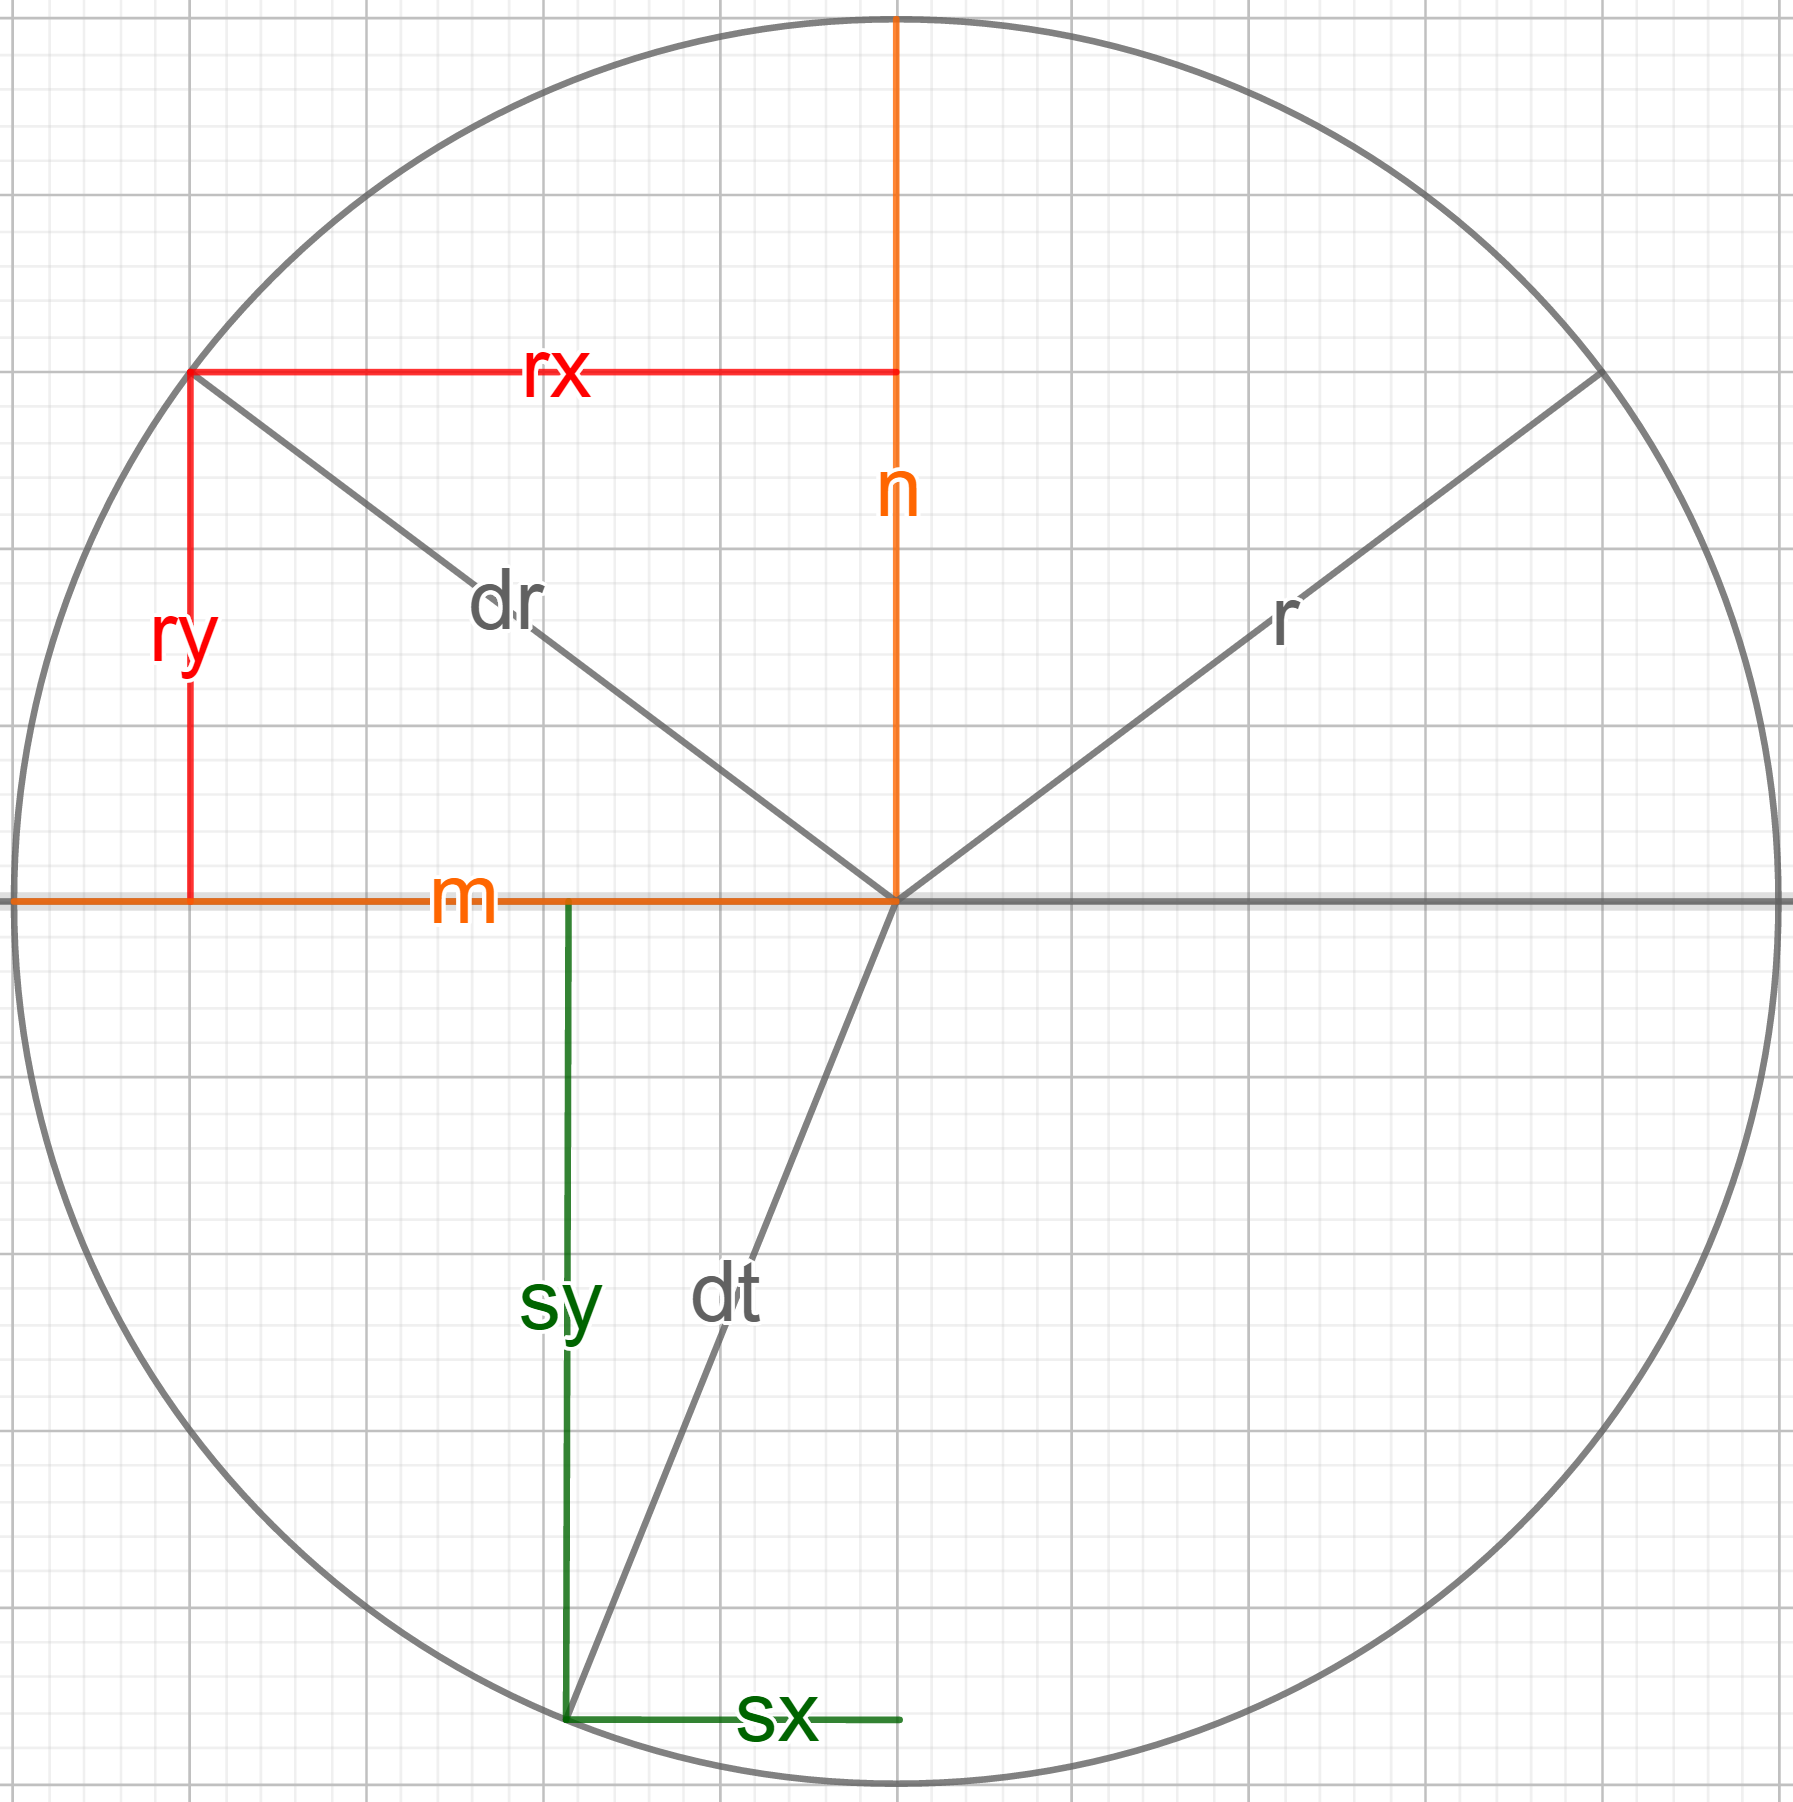
\includegraphics[width=0.5\textwidth]{./Images/reflect_refract.jpg}
\caption{Reflections and Refractions}
\label{fig:A}
\end{minipage}
\end{figure}

\subsection{Reflection}

The direction of the reflection ray can be calculated from the incoming ray $\vec{r}$ and the face normal $\vec{n}$ as follows

\begin{align}
\vec{dr} &= 2 \vec{ry} + \vec{r}\\
&= 2 \cos(\theta_1) \vec{n} + \vec{r}\\
&= 2 (-\vec{r} \cdot \vec{n}) \vec{n} + \vec{r}
\end{align}

with

\begin{align}
\vec{ry} &= \vec{n} \cos(\theta_1) = ( -\vec{r} \cdot \vec{n} ) \vec{n} \\
\vec{rx} &= \vec{n} \sin(\theta_1) = \vec{dr} - \vec{ry} = (-\vec{r} \cdot \vec{n}) \vec{n} + \vec{r} \\
\end{align}


\subsection{Refraction}

The direction of the transmitted refraction ray can be constructed as follows $\vec{dt} = \vec{tx} + \vec{ty}$.\cite{de2006reflections} The part along the x-axis is equal to

\begin{align}
\vec{tx} &= \vec{m} \sin(\theta_2) \\
&= \frac{\vec{r} + \vec{ry}}{\sin(\theta_1)} \sin(\theta_2) \\
&= \frac{\vec{r} + \cos(\theta_1) \vec{n}}{\sin(\theta_1)} \sin(\theta_2) \\
&= \frac{\vec{r} + (-\vec{r} \cdot \vec{n}) \vec{n}}{\sin(\theta_1)} \sin(\theta_2) \\
\end{align}

with snells law $n_2 \sin(\theta_2) = n_1 \sin(\theta_1)$ we get:

\begin{align}
\vec{tx} &= \frac{\eta_1}{\eta_2} \big( \vec{r} + (-\vec{r} \cdot \vec{n}) \vec{n} \big)
\end{align}

The part along the y-axis can be computed with the pythagorean theorem:

\begin{align}
\vec{ty}^2 &= \underbrace{ \vec{dt}^2 }_{=1} - \vec{tx}^2 \\
\Rightarrow \vec{ty} &= \vec{n} \sqrt{1 - \vec{tx}^2}
\end{align}

or equivalently by

\begin{align}
\vec{ty} &= \vec{n} \cos(\theta_2) \\
&= \vec{n} \sqrt{1 - \sin(\theta_2)^2} \\
&= \vec{n} \sqrt{1 - \Bigg( \frac{\eta_1}{\eta_2} \Bigg)^2 \sin(\theta_1)^2} \\
&= \vec{n} \sqrt{1 - \Bigg( \frac{\eta_1}{\eta_2} \Bigg)^2 \big(1 - \cos(\theta_1)^2 \big)} \\
&= \vec{n} \sqrt{1 - \Bigg( \frac{\eta_1}{\eta_2} \Bigg)^2 \big(1 - ( \vec{r} \vec{n} )^2 \big)} \\
&= \vec{n} \sqrt{1 - \vec{tx}^2}
\end{align}

So the transmitted ray is equal to:

\begin{align}
\vec{dt} &= \vec{tx} + \vec{ty} \\
&= \vec{tx} + \vec{n} \sqrt{1 - \vec{tx}^2}
\end{align}

\subsection{Diffuse Reflection}

In case of perfect diffuse reflection an inicdent light ray gets randomly reflected. We calculate the direction of the reflected ray with two random numbers $u_1,u_2$:

\begin{align}
\vec{dr} = \begin{pmatrix} \sqrt{1-u_2^2} \cos(2\pi u_1) \\ \sqrt{1-u_2^2} \sin(2\pi u_1) \\ u_2 \end{pmatrix}
\end{align}

where $\sqrt{1-u_2^2}$ and $u_2^2$ form a circle and $2\pi u_1$ sample the angle $\phi$ and produce a random vector on a half-sphere.

\subsection{Amount of reflections and transmission}
The amount of reflektion and transmission is described by fresnel laws. To avoid the long computation and averaging over the two polarizations we can use Schlicks approximation.

\begin{align}
R_0 = \Bigg( \frac{\eta_1 - \eta_2}{\eta_1 + \eta_2} \Bigg) ^2 \\
Re = R_0 + (1-R_0)(1-\cos(\theta_1)^2) \\
Tr = 1 - Re
\end{align}

The factor $R_0$ is equal to the minimum reflectivity of the medium, i.e. the reflectivity at direct incidence $\theta=0$ of light.

%press f11 and f1
\bibliographystyle{unsrt}
\bibliography{references}

\end{document}